\section{Lezione 6}
\subsection{Ripasso: simboli di Landau (\texorpdfstring{$o$}{o}-piccolo)}
\begin{definition}
    \label{def:5.4}
    Date $f\colon I \to \amsbb{R}$ e $g\colon I \to \amsbb{R}$ e $x_0\in\amsbb{R}$ un punto di accumulazione per $I$ (o eventualmente $+\infty$), diremo che $f$ \emph{è un $o$-piccolo di $g$ per $x\to x_0$}, scritto $f=o(g)$, se
    \[
    \lim_{x\to x_0} \frac{f(x)}{g(x)} = 0
    \]
\end{definition}
\subsection{Esercizi: limiti con i simboli di Landau}
\begin{exercise}
    \label{ex:5.4}
    Calcolare, se esiste,
    \[
    \lim_{x\to +\infty} \left(\sqrt[4]{1+   \arctan\left(\frac{5}{x^2}\right)}-\cos\left(\frac{3}{x}\right)\right)x^2
    \]
\end{exercise}
\begin{proof}[Soluzione]
    Notiamo che se definiamo $y = \frac{5}{x^2}$, abbiamo che $y\to 0$ in quanto $x\to +\infty$; di conseguenza, ricordando che, per $\xi\to 0$,
    \begin{tcolorbox}
    \[
    \underbrace{\arctan(\xi) = \xi+o(\xi)}_{\stepcounter{equation}\mbox{(\theequation)}} \qquad \underbrace{\sqrt[4]{1+\xi} = 1+\frac{\xi}{4}+o(\xi)}_{\stepcounter{equation}\mbox{(\theequation)}} \qquad \underbrace{\cos(\xi) = 1-\frac{\xi^2}{2}+o(\xi^2)}_{\stepcounter{equation}\mbox{(\theequation)}}
    \]
    \addtocounter{equation}{-3}\refstepcounter{equation}\label{eq:5.10}
    \addtocounter{equation}{0}\refstepcounter{equation}\label{eq:5.11}
    \addtocounter{equation}{0}\refstepcounter{equation}\label{eq:5.12}
    \end{tcolorbox}
    possiamo scrivere
    \[
    \begin{split}
        \sqrt[4]{1+\arctan\left(\frac{5}{x^2}\right)} & = \sqrt[4]{1+\arctan(y)} \overset{(\ref{eq:5.11})}{=} 1+\frac{\arctan(y)}{4}+o(\arctan(y)) \overset{(\ref{eq:5.10})}{=} \\
        & = 1 + \frac{y+o(y)}{4} + o(y+o(y)) = 1 + \frac{y}{4}+o(y)
    \end{split} 
    \]
    ove abbiamo usato il fatto che $\arctan(y)\to 0$ per $y\to 0$ e le proprietà dei simboli di Landau
    \[
    o(y+o(y)) = o(y) \qquad o(y)+o(y) = o(y)
    \]
    Riscrivendo in funzione di $x$ abbiamo che per $x\to +\infty$
    \[
    \sqrt[4]{1+\arctan\left(\frac{5}{x^2}\right)} = 1 + \frac{5}{4}\frac{1}{x^2} + o\left(\frac{1}{x^2}\right)
    \]
    Allo stesso modo, definendo $y=\frac{3}{y}$ abbiamo
    \[
    \cos\left(\frac{3}{x}\right) = \cos(y) \overset{(\ref{eq:5.12})}{=} 1-\frac{y^2}{2} + o(y^2)
    \]
    che riscritta in funzione di $x$ diventa
    \[
    \cos\left(\frac{3}{x}\right) = 1-\frac{9}{2}\frac{1}{x^2} + o\left(\frac{1}{x^2}\right) \ \text{per} \ x\to+\infty 
    \]
    Il limite diventa quindi
    \[
    \begin{split}
        & \lim_{x\to+\infty} \left(\sqrt[4]{1+   \arctan\left(\frac{5}{x^2}\right)}-\cos\left(\frac{3}{x}\right)\right)x^2 = \\
        & =  \lim_{x\to+\infty}\left(1+\frac{5}{4}\frac{1}{x^2} + o\left(\frac{1}{x^2}\right)-1+\frac{9}{2}\frac{1}{x^2}+o\left(\frac{1}{x^2}\right)\right)x^2 = \\
        & = \lim_{x\to+\infty}\left(\frac{5}{4}\frac{1}{x^2}+\frac{9}{2}\frac{1}{x^2} + o\left(\frac{1}{x^2}\right)\right)x^2 = \lim_{x\to+\infty} \frac{23}{4}+o\left(\frac{1}{x^2}\right)x^2
    \end{split}
    \]
    Ricordiamo che, per la definizione \ref{def:5.4}, una funzione $f$ è $o\left(\frac{1}{x^2}\right)$ per $x\to+\infty$ se
    \[
    \lim_{x\to+\infty}\frac{f(x)}{\frac{1}{x^2}} = \lim_{x\to+\infty}x^2 f(x) = 0
    \]
    Quindi 
    \[
    \lim_{x\to+\infty} o\left(\frac{1}{x^2}\right)x^2 = 0
    \]
    e di conseguenza
    \[
    \lim_{x\to +\infty} \left(\sqrt[4]{1+   \arctan\left(\frac{5}{x^2}\right)}-\cos\left(\frac{3}{x}\right)\right)x^2 = \frac{23}{4}
    \]
\end{proof}
\begin{exercise}
    \label{ex:5.5}
    Calcolare, se esiste,
    \[
    \lim_{x\to 0} \frac{1-e^{\cos(x)-1}}{\sqrt{\cos(\log(1+\sin(x)))}-1}
    \]
\end{exercise}
\begin{proof}[Soluzione]
    Per svolgere l'esercizio, consideriamo i seguenti sviluppi in termini di simboli di Landau per $\xi \to 0$: 
    \begin{tcolorbox}
    \[
    \!\!\!
    \underbrace{e^\xi= 1+\xi+o(\xi)}_{\stepcounter{equation}\mbox{(\theequation)}} \quad \underbrace{\log(1+\xi) = \xi + o(\xi)}_{\stepcounter{equation}\mbox{(\theequation)}} \quad \underbrace{\sin(\xi) = \xi + o(\xi)}_{\stepcounter{equation}\mbox{(\theequation)}} \quad \underbrace{\sqrt{1+\xi} = 1 + \frac{\xi}{2}+o(\xi)}_{\stepcounter{equation}\mbox{(\theequation)}}
    \]
    \addtocounter{equation}{-4}\refstepcounter{equation}\label{eq:5.13}
    \addtocounter{equation}{0}\refstepcounter{equation}\label{eq:5.14}
    \addtocounter{equation}{0}\refstepcounter{equation}\label{eq:5.15}
    \addtocounter{equation}{0}\refstepcounter{equation}\label{eq:5.16}
    \end{tcolorbox}
    Consideriamo separatamente numeratore e denominatore:
    \begin{enumerate}[(i)]
        \item Per il numeratore, notiamo che se definiamo $y= \cos(x)-1$ vale che $y\to 0$ per $x\to 0$; quindi
        \[
        \begin{split}
            e^{\cos(x)-1} & = e^y \overset{(\ref{eq:5.13})}{=} 1+y+o(y) = 1 + (\cos(x)-1) + o(\cos(x)-1) = \\
            & = \cos(x)+o(\cos(x)-1) \overset{(\ref{eq:5.12})}{=} 1-\frac{x^2}{2}+o(x^2) + o\left(1-\frac{x^2}{2}-1\right) = \\
            & = 1-\frac{x^2}{2}+o(x^2)
        \end{split}
        \]
        e di conseguenza per $x\to 0$ il numeratore è
        \[
        1-e^{\cos(x)-1} = 1-\left(1-\frac{x^2}{2}+o(x^2)\right) = \frac{x^2}{2} + o(x^2)
        \]
        \item Notiamo che $y=\sin(x)\to0$ per $x\to 0$, che $z = \log(1+y)\to 0$ per $y\to 0$ e che $\xi = \cos(z)-1\to 0$ per $z\to 0$; quindi
        \[
        \begin{split}
            & \sqrt{\cos(\log(1+\sin(x)))}-1 = \sqrt{1+(\cos(z)-1)}-1 = \sqrt{1+\xi} -1\overset{(\ref{eq:5.16})}{=}\\
            & = 1+\frac{\xi}{2} + o(\xi) -1 = \frac{\cos(z)-1}{2} + o(\cos(z)-1) \overset{(\ref{eq:5.12})}{=} \\
            & = \frac{1}{2}\left(1-\frac{z^2}{2}+o(z^2)-1\right)+o\left(\frac{z^2}{2}+o(z^2)\right) = -\frac{z^2}{4}+o(z^2) =\\
            & = -\frac{\log^2(1+y)}{4}+o(\log^2(1+y)) \overset{(\ref{eq:5.14})}{=} -\frac{(y+o(y))^2}{4} +o((y+o(y))^2) =  \\
            & = -\frac{y^2 +2yo(y)+o(y)^2}{4}+o(y^2 +2yo(y)+o(y)^2) = -\frac{y^2}{4}+o(y^2) = \\
            & = -\frac{\sin^2(x)}{4}+o(\sin^2(x)) \overset{(\ref{eq:5.15})}{=} -\frac{(x+o(x))^2}{4} + o((x+o(x))^2) = -\frac{x^2}{4}+o(x^2)
        \end{split}
        \]
    \end{enumerate}
    Quindi per $x\to 0$
    \[
    \frac{1-e^{\cos(x)-1}}{\sqrt{\cos(\log(1+\sin(x)))}-1} = \frac{\frac{x^2}{2}+o(x^2)}{-\frac{x^2}{4}+o(x^2)} = -\frac{\frac{x^2}{2}}{\frac{x^2}{4}}\frac{\left(1+2\frac{o(x^2)}{x^2}\right)}{\left(1-4\frac{o(x^2)}{x^2}\right)} = -2\frac{\left(1+2\frac{o(x^2)}{x^2}\right)}{\left(1-4\frac{o(x^2)}{x^2}\right)}
    \]
    Come prima, per definizione di $o$-piccolo, $\lim_{x\to 0} \frac{o(x^2)}{x^2} = 0$; di conseguenza, sfruttando i teoremi \ref{th:4.2}, \ref{th:4.3} e \ref{th:4.4} vale che
    \[
    \lim_{x\to 0} \frac{1-e^{\cos(x)-1}}{\sqrt{\cos(\log(1+\sin(x)))}-1} = \lim_{x\to 0}-2\frac{\left(1+2\frac{o(x^2)}{x^2}\right)}{\left(1-4\frac{o(x^2)}{x^2}\right)} = -2
    \]
\end{proof}
\subsection{Ripasso: derivabilità e differenziabilità, interpretazione geometrica della derivata}
\begin{definition}
    \label{def:6.1}
    Sia $f\colon(a,b)\to\amsbb{R}$, e sia $x\in(a,b)$; definiamo il \emph{rapporto incrementale di $f$ in $x$} come la funzione $\phi_x \colon (a,b) \setminus \{x\} \to \amsbb{R}$,
    \[
    \phi_x(t) = \frac{f(t)-f(x)}{t-x}
    \]
    Diremo che $f$ è \emph{derivabile in $x$} se esiste finito
    \begin{equation}
        \label{eq:6.1}
        \lim_{t\to x} \phi_x(t) = \lim_{t\to x} \frac{f(t)-f(x)}{t-x} = f'(x)
    \end{equation}
\end{definition}
\begin{remark}
    Detto $I\subseteq (a,b)$ l'insieme dei punti in cui $f$ è derivabile, possiamo definire una funzione $ I\ni x \mapsto f'(x)\in \amsbb{R}$, detta \emph{derivata prima} di $f$, che si indica con il simbolo $f'$.
\end{remark}
\begin{definition}
    \label{def:6.2}
    Dati $f\colon(a,b)\to\amsbb{R}$ e $x\in(a,b)$, diremo che $f$ è \emph{differenziabile in $x$} se esiste un'applicazione lineare $A_x\colon\amsbb{R}\to \amsbb{R}$ tale che
    \begin{equation}
        \label{eq:6.2}
        \lim_{\abs{h}\to0}\frac{\abs{f(x+h)-f(x)-A_x h}}{\abs{h}}=0
    \end{equation}
\end{definition}
\begin{remark}
    Ricordiamo che vale il teorema \ref{th:4.6}, e che quindi $\abs{h}\to 0$ se e solo se $h\to0$ e $\abs{f(h)}\to0$ se e solo se $f(h)\to0$. Possiamo quindi riscrivere la (\ref{eq:6.1}) come
    \[
    \lim_{h\to 0} \frac{f(x+h)-f(x)-A_x h}{h}=0
    \]
    Per la definizione \ref{def:5.4} vale quindi che
    \[
    f(x+h)-f(x)-A_xh = o(h) \iff f(x+h) = f(x) + A_x h+o(h)
    \]
    ossia $f$ è differenziabile in $x$ se in un intorno di $h$ possiamo approssimare $f$ con un'applicazione lineare $A_x$ commettendo un errore contenuto ($o(h)$).
\end{remark}
\begin{remark}
    Dai corsi di geometria sappiamo che, fissata una base di $\amsbb{R}$, esiste una corrispondenza biunivoca fra applicazioni lineari $A_x\in L(\amsbb{R}, \amsbb{R})$ e matrici $1\times 1$ a coefficienti reali, ossia numeri reali: in particolare, data l'applicazione lineare $A_x\colon \amsbb{R}\to\amsbb{R}$, esiste $m_{A_x}\in\amsbb{R}$ tale che
    \[
    A_x(h) = m_{A_x}h \ \text{per ogni} \ h\in\amsbb{R}
    \]
\end{remark}
\begin{theorem}
    \label{th:6.1}
    Data $f\colon (a,b)\to\amsbb{R}$, $f$ è differenziabile in $x$ se e solo se $f$ è derivabile in $x$.
\end{theorem}
\begin{proof}
    Dimostriamo le due implicazioni.
    \begin{enumerate}[(i)]
        \item Supponiamo che $f$ sia differenziabile in $x$, e mostriamo che $f$ è derivabile in $x$. Sappiamo che
        \[
        f(x+h)=f(x)+A_x h +o(h) = f(x)+m_{A_x}h +o(h)
        \]
        e di conseguenza
        \[
        \lim_{h\to 0} \frac{f(x+h)-f(x)}{h} = \lim_{h\to 0} \frac{f(x)+m_{A_x}h+o(h)-f(x)}{h} = m_{A_x}+\lim_{h\to 0} \frac{o(h)}{h} = m_{A_x} 
        \]
        Notiamo che il limite in (\ref{eq:6.1}) può essere scritto come
        \[
        \lim_{t\to x} \frac{f(t)-f(x)}{t-x} = \lim_{t\to x} \frac{f(t-x+x)-f(x)}{t-x}\overset{h=t-x}{=} \lim_{h\to 0} \frac{f(x+h)-f(x)}{h}
        \]
        in quanto $h\to 0$ se $t\to x$. Abbiamo quindi che il limite (\ref{eq:6.1}) esiste finito, e che $f'(x) = m_{A_x}$.
        \item Supponiamo ora che $f$ sia derivabile in $x$ e mostriamo che $f$ è differenziabile in x. Per definizione vale che
        \[
        \lim_{t\to x}\frac{f(t)-f(x)}{t-x} = \lim_{h\to 0}\frac{f(x+h)-f(x)}{h} = f'(x)
        \]
        ossia
        \[
        \lim_{h\to 0}\frac{f(x+h)-f(x)}{h}-f'(x) = 0
        \]
        Possiamo riscrivere il precedente limite come
        \[
        0=\lim_{h\to 0}\frac{f(x+h)-f(x)}{h}-f'(x) = \lim_{h\to 0} \frac{f(x+h)-f(x)-f'(x)h}{h}
        \]
        Per il teorema \ref{th:4.6} sappiamo che 
        \[
        \lim_{h\to 0}\abs{\frac{f(x+h)-f(x)-f'(x)h}{h}} = \lim_{h\to 0} \frac{\abs{f(x+h)-f(x)-f'(x)h}}{\abs{h}}=0
        \]
        e di conseguenza l'applicazione lineare $\amsbb{R}\ni h \mapsto f'(x)h$ indotta da $f'(x)\in\amsbb{R}$ soddisfa la definizione \ref{def:6.2}.
    \end{enumerate}
\end{proof}
\begin{remark}
    Questo teorema ci dice che per funzioni $f\colon \amsbb{R}\to \amsbb{R}$ differenziabilità e derivabilità sono due concetti equivalenti. Non è così per funzioni $f\colon \amsbb{R}^n\to \amsbb{R}$! Ci sono esempi\footnote{Ad esempio, la funzione $\amsbb{R}^2\ni (x,y)\mapsto \frac{x^2y}{x^2+y^2}$ per $(x,y)\ne (0,0)$ e $f(0,0)=0$ è derivabile (direzionalmente) in $(0,0)$ ma non è differenziabile.} di funzioni derivabili ma non differenziabili.
\end{remark}
\begin{theorem}
    \label{th:6.2}
    Siano $f,g\colon (a,b)\to \amsbb{R}$ due funzioni differenziabili in $x\in(a,b)$; allora
    \begin{enumerate}[(i)]
        \item $(f+g)'(x) = f'(x) + g'(x)$;
        \item $(\lambda f)'(x) = \lambda f'(x)$;
        \item (Regola di Leibniz)
        \begin{equation}
            \label{eq:6.3}
            (fg)'(x) = f'(x)g(x) + f(x)g'(x)
        \end{equation}
    \end{enumerate}
    Inoltre, se $g\colon (c,d) \to \amsbb{R}$ è tale per cui $f((a,b))\subseteq (c,d)$ e $g$ è differenziabile in $f(x)\in(c,d)$, allora $g\circ f \colon (a,b) \to \amsbb{R}$ è differenziabile in $x$ e vale la regola della catena
    \begin{equation}
        \label{eq:6.4}
        (g\circ f)'(x) = g'(f(x))f'(x)
    \end{equation}
\end{theorem}
\begin{example}
    Consideriamo la funzione $f\colon\amsbb{R}\to \amsbb{R}$,
    \[
    f(x) = \begin{dcases}
        x^2\sin\left(\frac{1}{x}\right)\, & x\ne 0\\
        0\, & x=0
    \end{dcases}
    \]
    e cerchiamo di determinare l'insieme $I\subseteq \amsbb{R}$ in cui è differenziabile. In $\amsbb{R}\setminus\{0\}$ la funzione è prodotto e composizione di funzioni differenziabili, e quindi per il teorema \ref{th:6.2} vale che $f$ è differenziabile in $\amsbb{R}\setminus \{0\}$, e la sua derivata prima in $\amsbb{R}\setminus\{0\}$ è data da
    \[
    \begin{split}
        f'(x) & = \frac{d}{dx}\left(x^2 \sin\left(\frac{1}{x}\right)\right) \overset{(\ref{eq:6.3})}{=} 2x\sin\left(\frac{1}{x}\right) + x^2 \frac{d}{dx}\left(\sin\left(\frac{1}{x}\right)\right) \overset{(\ref{eq:6.4})}{=} \\
        & = 2x\sin\left(\frac{1}{x}\right)+x^2 \cos\left(\frac{1}{x}\right)\left(-\frac{1}{x^2}\right) = 2x\sin\left(\frac{1}{x}\right)-\cos\left(\frac{1}{x}\right)
    \end{split}
    \]
    Per la derivabilità in $0$, bisogna considerare invece il rapporto incrementale (\ref{eq:6.1}),
    \[
    \phi_0(t) = \frac{f(t)-f(0)}{t-0} = \frac{1}{t}t^2\sin\left(\frac{1}{t}\right) = t\sin\left(\frac{1}{t}\right)
    \]
    e calcolare $\lim_{t\to 0} \phi_0(t)$. Notiamo che, poiché $\abs{\sin(x)}\le 1$ per ogni $x\in\amsbb{R}$,
    \[
    0\le \abs{\phi_0(t)}= \abs{t\sin\left(\frac{1}{t}\right)} \le \abs{t}
    \]
    e quindi per il teorema \ref{th:4.5} vale che $\abs{\phi_0(t)}\to 0$ per $t\to 0$, e per il teorema \ref{th:4.6} vale che
    \[
    \lim_{t\to 0} \phi_0(t) = 0 = f'(0)
    \]
    Quindi $f$ è derivabile su tutto $\amsbb{R}$, e
    \[
    f'(x) = \begin{dcases}
        2x\sin\left(\frac{1}{x}\right)-\cos\left(\frac{1}{x}\right)\, & x\ne 0\\
        0\, & x=0
    \end{dcases}
    \]
    Notiamo che $f'$ è continua in $\amsbb{R}\setminus\{0\}$, essendo composizione e prodotto di funzioni continue,  ma non è continua in $0$: infatti, considerando le due successioni
    \[
    a_n = \frac{1}{2n\pi} \qquad b_n = \frac{1}{(2n+1)\pi}
    \]
    che tendono a $0$ per $n\to\infty$ vale che
    \[
    \lim_{n\to\infty} f'(a_n) = \frac{1}{2n\pi}\sin(2n\pi))-\cos(2n\pi) = \lim_{n\to\infty} -\cos(2n\pi) = -1
    \]
    e che
    \[
    \lim_{n\to\infty} f'(b_n) = \frac{1}{(2n+1)\pi}\sin((2n+1)\pi))-\cos((2n+1)\pi) = \lim_{n\to\infty} -\cos((2n+1)\pi) = 1
    \]
    Per il teorema \ref{th:5.1} quindi $\lim_{t\to 0} f'(t)$ non esiste, e quindi $f'$ non può essere continua in 0.
\end{example}
Data una funzione $f\colon(a,b)\to\amsbb{R}$, sappiamo che $f$ è derivabile in $x_0\in(a,b)$ se 
\[
f(x_0+h) -f(x_0) = f'(x_0)h+o(h)
\]
Consideriamo quindi $F\colon h\mapsto f(x_0+h)-f(x_0)$; sappiamo che
\[
F(h) = f'(x_0)h +o(h)
\]
ossia $h\mapsto f'(x_0)h$ è l'applicazione lineare che meglio approssima $F$ in prossimità dell'origine.
\begin{center}
    \begin{minipage}{.45\linewidth}
        \centering
        \begin{tikzpicture}[scale=1.3, font=\footnotesize]
            \tzaxes(-1.2,-1.2)(4,2.4){$x$}[b]
            \tzfn[blue]"curve"{cos(3*deg(\x))+sin(.9*deg(\x))}[-.5:3.3]{$f(x)$}[b]
            \tzproj(1.5, 0.7649){$x_0$}{$f(x_0)$}
        \end{tikzpicture}
    \end{minipage}
    \hspace{1pt}
    \begin{minipage}{.45\linewidth}
        \centering
        \begin{tikzpicture}[scale=1.3, font=\footnotesize]
            \tzaxes(-2.7,-1.9)(2.5,1.7){$h$}[b]
            \tzfn[red]"curve"{cos(3*deg(\x+1.5))+sin(.9*deg(\x+1.5))-0.7649}[-2:1.8]{$F(h)$}[b]
            \tzfn[teal]"line"{3.1297*\x}[-.5:.5]{$y=f'(x_0)h$}[r]
        \end{tikzpicture}
    \end{minipage}
\end{center}
Notiamo che il grafico, riportato a destra, di $F$, altro non è se non il grafico di $f(x)$ traslato di $(-x_0, -f(x_0))$: infatti, se consideriamo la coppia $(h, F(h))$ e la trasliamo di $(x_0, f(x_0))$ otteniamo
\[
(h, F(h)) \longrightarrow (h+x_0, F(h)+f(x_0)) = (h+x_0, f(h+x_0))
\]
Possiamo sempre scrivere $h=x-x_0$ per un qualche $x\in\amsbb{R}$; di conseguenza il punto $(h, F(h))$ viene mandato dalla traslazione in $(x,f(x))$. Poiché $h$ scorre su tutto $\amsbb{R}$, così fa $x$, e quindi abbiamo
\[
\{(h, F(h)), \ h\in\amsbb{R}\}\longrightarrow \{(x, f(x)), \ x\in\amsbb{R}\}
\]
Consideriamo invece la retta $\{(h, f'(x_0)h), \ h\in\amsbb{R}\}$: la traslazione rigida per il vettore $(x_0, f(x_0))$ agisce come
\[
(h, f'(x_0)h)\longrightarrow (h+x_0, f'(x_0)h+f(x_0))
\]
e scrivendo $h=x-x_0$ come fatto precedentemente otteniamo
\[
(h, f'(x_0)h)\longrightarrow (x, f'(x_0)(x-x_0) + f(x_0))
\]
Quindi
\[
\{(h, f'(x_0)h), \ h\in\amsbb{R}\} \longrightarrow \underbrace{\{(x, f'(x_0)(x-x_0)+f(x_0)), \ x\in\amsbb{R}\}}_{\text{retta passante per }(x_0, f(x_0)) \ \text{con coeff. angolare} \ f'(x_0)}
\]
ossia la retta che meglio approssima la funzione $F$ in un intorno dell'origine viene trasformata nella retta che meglio approssima il grafico della funzione $f$ in un intorno del punto $(x_0, f(x_0))$. La derivata prima $f'(x_0)$ è il coefficiente angolare di questa retta; ora, dalla definizione \ref{def:6.1} e dall'equazione (\ref{eq:6.1}) sappiamo che
\[
f'(x_0) = \lim_{t\to x_0} \frac{f(t)-f(x_0)}{t-x_0}
\]
ossia per calcolare $f'(x_0)$ stiamo considerando il coefficiente angolare della secante passante per i punti $(x_0, f(x_0))$ e $(t, f(t))$ e ne valutiamo il comportamento nel limite in cui i due punti coincidono; possiamo cioè immaginarci di tendere alla retta tangente al grafico di $f(x)$ nel punto $(x_0, f(x_0))$. Alla luce della precedente discussione, nel caso in cui $f$ sia differenziabile in $x_0$ possiamo quindi definire la retta tangente come 
\[
\{(x, f'(x_0)(x-x_0)+f(x_0)), \ x\in\amsbb{R}\}
\]
\begin{example}
    Consideriamo la funzione $f(x) = \log(\arctan(x^2))$; vogliamo determinarne l'equazione della retta tangente al grafico di $f(x)$ nel punto $\left(1, \log\left(\frac{\pi}{4}\right)\right)$. Per quanto detto precedentemente, sappiamo che questa è definita da
    \[
    \left\{\left(x, f'(1)(x-1)+\log\left(\frac{\pi}{4}\right)\right), \ x\in\amsbb{R}\right\}
    \]
    Dobbiamo quindi calcolare $f'(1)$:
    \[
    \begin{split}
        f'(1) & = \frac{d}{dx}f(x)\bigg|_{x=1} = \frac{d}{dx}\left(\log(\arctan(x^2))\right)\bigg|_{x=1}\overset{(\ref{eq:6.4})}{=}\left(\frac{1}{\arctan(x^2)}\frac{1}{1+x^2}2x\right)\bigg|_{x=1} =\\
        & = \frac{1}{\arctan(1)} = \frac{4}{\pi}
    \end{split}
    \]
    L'equazione della retta tangente al grafico di $f$ in $\left(1, \log\left(\frac{\pi}{4}\right)\right)$ è quindi data da
    \[
    y = \frac{4}{\pi}(x-1)+\log\left(\frac{\pi}{4}\right) = \frac{4}{\pi}x+\log\left(\frac{\pi}{4}\right) - \frac{4}{\pi} 
    \]
    \begin{center}
        \begin{tikzpicture}[scale=1.5, font=\footnotesize]
            \tzaxes(0,-2)(4,2){$x$}[b]
            \tzfn[blue]"curve"{ln(rad(atan(\x*\x))))}[0.4:3.5]{$\log(\arctan(x))$}[b]
            \tzfn[red]"curve"{1.2732*\x -0.2416-1.2732}[0.4:2]{$\frac{4}{\pi}(x-1)+\log\left(\frac{\pi}{4}\right)$}[ar]
            \tzprojx(1, -0.2416){$1$}[a]
            \tzprojy(1, -0.2416){$\log\left(\frac{\pi}{4}\right)$}[l]
        \end{tikzpicture}
    \end{center}
    Se avessimo invece voluto sapere l'equazione della retta tangente al grafico di $f^{-1}(x)$ nel punto $\left(\log\left(\frac{\pi}{4}\right), 1\right)$?\\
    Notiamo innanzitutto che $f\colon\amsbb{R}\setminus\{0\} \to \amsbb{R}$ è pari; pertanto questa non è iniettiva su $\amsbb{R}\setminus\{0\}$. Possiamo però restringerci a $f\colon \amsbb{R}^+\to \amsbb{R}$; in questo caso notiamo che $\log(\cdot)\colon \amsbb{R}^+\to \amsbb{R}$ è monotona strettamente crescente, e lo stesso vale per $\arctan(\cdot)\colon \amsbb{R}^+\to\amsbb{R}$; pertanto
    \[
    f(x)<f(y) \iff x<y \ \text{su} \ \amsbb{R}^+
    \]
    e l'iniettività segue. Per quanto riguarda la suriettività, notiamo che
    \[
    \lim_{x\to +\infty} f(x) = \log\left(\frac{\pi}{2}\right) \qquad \lim_{x\to 0^+} f(x) = -\infty
    \]
    e che $f$ è continua, essendo composizione di funzioni continue; vale pertanto il teorema dei valori intermedi \ref{th:5.3}: di conseguenza $f\colon \amsbb{R}^+ \to \left(-\infty, \log\left(\frac{\pi}{2}\right)\right)$ è iniettiva e suriettiva, e pertanto invertibile. \\
    A questo punto, la retta tangente al grafico di $f^{-1}$ in $\left(\log\left(\frac{\pi}{4}, 1\right)\right)$ sarà data da
    \[
    \left\{\left(x, (f^{-1})'\left(\log\left(\frac{\pi}{4}\right)\right)\left(x-\log\left(\frac{\pi}{4}\right)\right)+1\right), \ x\in\amsbb{R}\right\}
    \]
    Per calcolare $(f^{-1})'\left(\log\left(\frac{\pi}{4}\right)\right)$ abbiamo diverse possibilità:
    \begin{enumerate}[(i)]
        \item Ci ricordiamo che vale la regola della catena (\ref{eq:6.4}), ossia se $f$ è derivabile in $x$ e $f^{-1}$ è derivabile in $f(x)$ vale che
        \[
        \frac{d}{dx}(x) = \frac{d}{dx}(f^{-1}(f(x)) = (f^{-1})'(f(x)) f'(x) 
        \]
        Notiamo che se $f'(x) = 0$ non possiamo usare questo metodo per calcolare $(f^{-1})'(f(x))$; se invece $f'(x)\ne 0$ vale che
        \[
        (f^{-1})'(f(x)) = \frac{1}{f'(x)} \iff (f^{-1})'(y) = \frac{1}{f'(f^{-1}(y))}
        \]
        Nel nostro caso vale che $f'(1) \ne 0$, e quindi
        \[
        (f^{-1})'\left(\log\left(\frac{\pi}{4}\right)\right) = \frac{1}{f'(1)} = \frac{\pi}{4}
        \]
        e quindi l'equazione della retta tangente al grafico di $f^{-1}$ in $\left(\log\left(\frac{\pi}{4}\right), 1\right)$ è data da
        \[
        y=\frac{\pi}{4}x+1 - \frac{\pi}{4}\log\left(\frac{\pi}{4}\right)
        \]
        \item Osserviamo le equazioni delle due rette:
        \[
        y=\frac{4}{\pi}x + \log\left(\frac{\pi}{4}\right)-\frac{4}{\pi} \qquad y=\frac{\pi}{4}x+1 - \frac{\pi}{4}\log\left(\frac{\pi}{4}\right)
        \]
        Notiamo che se nella prima scambiamo $x$ e $y$ ottenendo
        \[
        x=\frac{4}{\pi}y+\log\left(\frac{\pi}{4}\right)-\frac{4}{\pi}
        \]
        ed esplicitiamo la $y$ in funzione di $x$ otteniamo
        \[
        x- \log\left(\frac{\pi}{4}\right)+\frac{4}{\pi} = \frac{4}{\pi}y \iff y = \frac{\pi}{4}x-\frac{\pi}{4}\log\left(\frac{\pi}{4}\right)+1
        \]
        cioè la seconda equazione.\\
        Perché funziona? Supponiamo di avere una funzione $f\colon D_f\to I_f$ invertibile; la sua funzione $f^{-1}\colon D_{f^{-1}}\to I_{f^{-1}}$ avrà grafico
        \[
        \text{Graph}(f^{-1}) = \left\{(x, f^{-1}(x))\in\amsbb{R}^2, \ x\in D_{f^{-1}}\right\}
        \]
        Ricordiamo che nel caso di funzioni invertibili $D_{f^{-1}} = I_f$; quindi per ogni $x\in D_{f^{-1}}$ esiste un unico $t\in D_f$ tale che $x=f(t)$; quindi
        \[
        \text{Graph}(f^{-1}) = \left\{(f(t), f^{-1}(f(t))), \ t\in D_f\right\} = \left\{(f(t), t), \ t\in D_f\right\} 
        \]
        ossia possiamo disegnare il grafico di $f^{-1}$ tracciando il grafico di $f$ invertendo gli assi. Supponiamo ora che la retta
        \[
        r = \{(t, r(t)), \ x\in\amsbb{R}\}
        \]
        sia tangente al grafico di $f$ in $(t_0, f(t_0))$; allora necessariamente la retta
        \[
        r'=\{(r(t), t), \ t\in\amsbb{R} \}
        \]
        sarà tangente a
        \[
        \left\{(f(t), t), \ t\in D_f\right\} = \left\{(x, f^{-1}(x)), \ x\in D_{f^{-1}}\right\} = \text{Graph}(f^{-1})
        \]
        in $(f(t_0), t_0)$.
        \item Talvolta possiamo calcolare direttamente $f^{-1}(x)$; in questo caso ad esempio la funzione inversa $f^{-1}\colon \left(-\infty, \log\left(\frac{\pi}{2}\right)\right)\to\amsbb{R}^+$ è data da
        \[
        f^{-1}(x) = \sqrt{\tan(e^{x})}
        \]
        A questo punto è sufficiente derivare $f^{-1}$ per calcolare la derivata prima in $\log\left(\frac{\pi}{4}\right)$:
        \[
        \frac{d}{dx}f^{-1}(x))\bigg|_{x=\log\left(\frac{\pi}{4}\right)} = \frac{1}{2}\frac{1}{\sqrt{\tan(e^x)}}\frac{1}{\cos^2(e^x)}e^x\bigg|_{x=\log\left(\frac{\pi}{4}\right)} = \frac{1}{2}\frac{4}{2}\frac{\pi}{4} = \frac{\pi}{4}
        \]
        e procedere come prima.
    \end{enumerate}
\end{example}
\subsection{Esercizi: derivabilità e differenziabilità}
\begin{exercise}
    \label{ex:6.1}
    Data la funzione
    \[
    f(x) = \begin{dcases}
        \alpha(\beta x + \alpha)^3\, & x\le 0\\
        2e^{\beta x} - \pi \cos\left(\frac{2\alpha}{\pi} x\right)\, & x>0
    \end{dcases}
    \]
    determinare i valori di $\alpha, \beta \in\amsbb{R}$ tali che $f$ sia differenziabile in 0.
\end{exercise}
\begin{proof}[Soluzione]
    Ricordiamo il seguente risultato
    \begin{tcolorbox}
        \begin{theorem}
            \label{th:6.3}
            Se $f\colon (a,b)\to\amsbb{R}$ è differenziabile in $x\in(a,b)$, allora $f$ è continua in $x$.
        \end{theorem}
    \end{tcolorbox}
    che è equivalente a
    \begin{tcolorbox}
        Se $f\colon (a,b)\to\amsbb{R}$ non è continua in $x\in(a,b)$, allora $f$ non è differenziabile in $x$.
    \end{tcolorbox}
    Cerchiamo allora per quali valori dei parametri la funzione è continua in $x=0$, ricordando che vale il teorema \ref{th:5.2}: dobbiamo quindi verificare che
    \[
    \lim_{x\to 0^+} f(x) = \lim_{x\to 0^-} f(x) = f(0) = \alpha^4
    \]
    Sicuramente per la continuità delle funzioni che contribuiscono alla definizione di $f$ in $(-\infty, 0]$ vale che
    \[
    \lim_{x\to 0^-}f(x) = \alpha^4
    \]
    Consideriamo quindi $\lim_{x\to 0^+} f(x)$: poiché le funzioni che definiscono $f$ in $(0, +\infty)$ sono la restrizione a questo intervallo illimitato di funzioni continue su tutto $\amsbb{R}$, vale che
    \[
    \lim_{x\to 0^+} f(x) = \lim_{x\to 0^+} 2e^{\beta x} - \pi \cos\left(\frac{2\alpha}{\pi} x\right) = 2e^0-\pi \cos(0) = 2-\pi
    \]
    Per avere una funzione continua dobbiamo quindi trovare i valori del parametro $\alpha$ tali che
    \[
    \alpha^4 = 2-\pi
    \]
    Questa equazione però non ha soluzioni in $\amsbb{R}$, in quanto $2-\pi<0$. Pertanto non esiste scelta dei parametri $\alpha,\beta$ tale da rendere $f$ differenziabile in $0$.
\end{proof}
\begin{remark}
    L'unico legame fra continuità e differenziabilità è quello descritto nel teorema \ref{th:6.3}. Il fatto che una funzione sia continua non implica nulla sul fatto che una funzione sia derivabil: esistono infatti esempi di funzioni continue su tutto $\amsbb{R}$ non derivabili in nessun punto (\cite[Teorema 7.18]{rudin1976principles}).
\end{remark}
\begin{exercise}
    \label{ex:6.2}
    Data la funzione
    \[
    f(x) = \begin{dcases}
        \alpha\sin(\pi e^{\beta(x-e)})+\beta\, & x\le e\\
        (x-e)^3-\alpha e^{-\alpha(x-e)}\, & x>e
    \end{dcases}
    \]
    determinare i valori di $\alpha, \beta\in\amsbb{R}$ tali che $f$ sia differenziabile in $e$.
\end{exercise}
\begin{proof}[Soluzione]
    Come prima, alla luce del teorema \ref{th:6.3} verifichiamo per quali valori dei parametri $f$ è continua in $e$, e grazie al teorema \ref{th:5.2} possiamo vedere se
    \[
    \lim_{x\to e^+} f(x) = \lim_{x\to e^-} f(x) = f(e) = \beta
    \]
    Poiché $f\colon (-\infty, e]\to \amsbb{R}$ è data dalla restrizione di $\alpha\sin(\pi e^{\beta(x-e)})+\beta$, che è composizione di funzioni continue su tutto $\amsbb{R}$, vale che
    \[
    \lim_{x\to e^-}f(x) = f(e) = \beta
    \]
    Per quanto riguarda $f\colon (e, +\infty)$, anche in questo caso $f$ è data dalla restrizione all'intervallo di funzioni continue su tutto $\amsbb{R}$; quindi
    \[
    \lim_{x\to e^+}f(x) = \lim_{x\to e^+} (x-e)^3-\alpha e^{-\alpha (x-e)} = -\alpha
    \]
    Quindi affinché $f$ sia continua in $e$ deve valere che $\beta = -\alpha$.\\
    Per quanto riguarda invece la differenziabilità, in questo caso possiamo operare in due modi diversi:
    \begin{enumerate}[(i)]
        \item Possiamo usare la definizione \ref{def:6.1}, in particolare l'equazione (\ref{eq:6.1}), e il teorema \ref{th:5.2} per dire che $f$ è differenziabile in $e$ se
        \[
        \underbrace{\lim_{t\to e^+}\frac{f(t)-f(e)}{t-e}}_{\stepcounter{equation}\mbox{(\theequation)}} = \underbrace{\lim_{t\to e^-}\frac{f(t)-f(e)}{t-e}}_{\stepcounter{equation}\mbox{(\theequation)}}
        \]
        \addtocounter{equation}{-2}\refstepcounter{equation}\label{eq:6.5}
        \addtocounter{equation}{0}\refstepcounter{equation}\label{eq:6.6}
        ed entrambi i limiti esistono finiti. Consideriamo il limite (\ref{eq:6.5}): ricordando che necessariamente $\alpha=-\beta$,
        \[
        \begin{split}
            &\lim_{x\to e^+} \frac{f(x)-f(e)}{x-e} = \lim_{x\to e^+} \frac{(x-e)^3 - \alpha e^{-\alpha(x-e)}-\beta}{x-e} \overset{t=x-e}{=} \\
            & = \lim_{t\to 0^+} \frac{t^3-\alpha e^{-\alpha t}-\beta}{t} \overset{(\ref{eq:5.13})}{=} \lim_{t\to 0^+} \frac{t^3-\alpha(1-\alpha t + o(t))+\alpha}{t} = \\
            & = \lim_{t\to 0^+} t^2 +\alpha^2 + \frac{o(t)}{t} = \alpha^2
        \end{split}
        \]
        Allo stesso modo, se consideriamo il limite (\ref{eq:6.6}) abbiamo che
        \[
        \begin{split}
            & \lim_{x\to e^-} \frac{f(x)-f(e)}{x-e} = \lim_{x\to e^-}\frac{\alpha\sin(\pi e^{\beta(x-e)})+\beta-\beta}{x-e} = \lim_{x\to e^-} \frac{\alpha\sin(\pi e^{\beta(x-e)}+\pi -\pi)}{x-e} = \\
            & = \lim_{x\to e^-} \frac{-\alpha\sin(\pi e^{\beta(x-e)}-\pi)}{x-e}= \overset{t=e^{\beta(x-e)}-1}{=} \lim_{t\to 0^-} \frac{-\alpha\sin(\pi t)}{\frac{1}{\beta}\log(1+t)} \overset{(\ref{eq:5.15})+(\ref{eq:5.14})}{=} \\
            & = \lim_{t\to 0^-} -\alpha\frac{-\alpha\pi t +o(t)}{t+o(t)} = -\alpha\lim_{t\to 0^-} \frac{-\alpha \pi t}{t}\frac{1+\frac{o(t)}{t}}{1+\frac{o(t)}{t}} = \pi \alpha^2 \lim_{t\to 0^-} \frac{1+\frac{o(t)}{t}}{1+\frac{o(t)}{t}} = \pi \alpha^2
        \end{split}
        \]
        ove abbiamo usato il teorema \ref{th:4.4} e la definizione \ref{def:5.4}. Quindi $f$ è differenziabile in $e$ se
        \[
        \begin{dcases}
            \alpha^2 = \pi \alpha^2 \\
            \beta = -\alpha 
        \end{dcases} \iff \alpha = \beta = 0
        \]
        \item Notiamo che $f$ è derivabile separatamente nei due tratti $(-\infty, e)$ e $(e, +\infty)$. Possiamo quindi provare a derivare $f$ separatamente nei due tratti, ottenendo una funzione
        \[
        f'(x) = \begin{dcases}
            \alpha \cos(\pi e^{\beta(x-e)})\pi \beta e^{\beta(x-e)}\, & x<e\\
            3(x-e)^2 + \alpha^2 e^{-\alpha(x-e)}\, & x>e
        \end{dcases}
        \]
        Resta da capire cosa succede nel punto $x=e$. Se consideriamo il limite sinistro del rapporto incrementale abbiamo che
        \[
        \lim_{t\to e^-} \frac{f(t)-f(e)}{t-e} = \lim_{t\to e^-}\frac{(\alpha\sin(\pi e^{\beta(t-e)})+\beta)-(\alpha\sin(\pi e^{\beta(e-e)})+\beta)}{t-e}
        \]
        Notiamo che la funzione $\alpha\sin(\pi e^{\beta(x-e)})+\beta$ è derivabile su tutto $\amsbb{R}$, e la sua derivata è continua; pertanto
        \[
        \begin{split}
            &\lim_{t\to e^-}\frac{(\alpha\sin(\pi e^{\beta(t-e)})+\beta)-(\alpha\sin(\pi e^{\beta(e-e)})+\beta)}{t-e} = \frac{d}{dt}\left(\alpha\sin(\pi e^{\beta(t-e)})+\beta\right)\bigg|_{t=e} = \\
            & = \lim_{t\to e^-} \frac{d}{dt}\left(\alpha\sin(\pi e^{\beta(t-e)})+\beta\right)
        \end{split}
        \]
        Quindi vale che
        \[
        \lim_{t\to e^-} \frac{f(t)-f(e)}{t-e} = \lim_{t\to e^-} f'(t)
        \]
        Dato che abbiamo imposto che $f$ sia continua in $e$ con $\beta = -\alpha$, vale che 
        \[
        f(e) = \lim_{x\to e^+} (x-e)^3-\alpha e^{-\alpha(x-e)} = (e-e)^3-\alpha e^{-\alpha(e-e)}
        \]
        Procedendo come prima si può quindi mostrare che
        \[
        \lim_{t\to e^+} \frac{f(t)-f(e)}{t-e} = \lim_{t\to e^+}f'(t)
        \]
        Se calcoliamo i due limiti, per la continuità delle funzioni abbiamo
        \[
        \lim_{t\to e^-}f'(t) = \lim_{t\to e^-} \alpha \cos(\pi e^{\beta(t-e)})\pi \beta e^{\beta(t-e)} = \alpha \cos(\pi) \pi \beta = \pi\alpha^2
        \]
        e 
        \[
        \lim_{t\to e^+} f'(t) = \lim_{t\to e^+} 3(t-e)^2 + \alpha^2 e^{-\alpha(t-e)} = \alpha^2
        \]
        Ci siamo quindi ricondotti allo stesso sistema
        \[
        \begin{dcases}
            \alpha^2 = \pi \alpha^2\\
            \beta = - \alpha
        \end{dcases} \iff \alpha=\beta = 0
        \]
    \end{enumerate}
\end{proof}
\newpage